\documentclass[a4paper,11pt]{article}
\usepackage{amsmath,amsthm,amsfonts,amssymb,amscd,amstext,vmargin,graphics,graphicx,tabularx,multicol} \usepackage[french]{babel}
\usepackage[utf8]{inputenc}  
\usepackage[T1]{fontenc} 
\usepackage[T1]{fontenc}
\usepackage{amsmath,amssymb}
\usepackage{pstricks-add,tikz,tkz-tab,variations}
\usepackage[autolanguage,np]{numprint} 
\usepackage{color}
\usepackage{ulem}

\setmarginsrb{1.5cm}{0.5cm}{1cm}{0.5cm}{0cm}{0cm}{0cm}{0cm} %Gauche, haut, droite, haut
\newcounter{numexo}
\newcommand{\exo}[1]{\stepcounter{numexo}\noindent{\bf Exercice~\thenumexo} : \marginpar{\hfill /#1}}
\reversemarginpar


\newcounter{enumtabi}
\newcounter{enumtaba}
\newcommand{\q}{\stepcounter{enumtabi} \theenumtabi.  }
\newcommand{\qa}{\stepcounter{enumtaba} (\alph{enumtaba}) }
\newcommand{\initq}{\setcounter{enumtabi}{0}}
\newcommand{\initqa}{\setcounter{enumtaba}{0}}

\newcommand{\be}{\begin{enumerate}}
\newcommand{\ee}{\end{enumerate}}
\newcommand{\bi}{\begin{itemize}}
\newcommand{\ei}{\end{itemize}}
\newcommand{\bp}{\begin{pspicture*}}
\newcommand{\ep}{\end{pspicture*}}
\newcommand{\bt}{\begin{tabular}}
\newcommand{\et}{\end{tabular}}
\renewcommand{\tabularxcolumn}[1]{>{\centering}m{#1}} %(colonne m{} centrée, au lieu de p par défault) 
\newcommand{\tnl}{\tabularnewline}

\newcommand{\trait}{\noindent \rule{\linewidth}{0.2mm}}
\newcommand{\hs}[1]{\hspace{#1}}
\newcommand{\vs}[1]{\vspace{#1}}

\newcommand{\N}{\mathbb{N}}
\newcommand{\Z}{\mathbb{Z}}
\newcommand{\R}{\mathbb{R}}
\newcommand{\C}{\mathbb{C}}
\newcommand{\Dcal}{\mathcal{D}}
\newcommand{\Ccal}{\mathcal{C}}
\newcommand{\mc}{\mathcal}

\newcommand{\vect}[1]{\overrightarrow{#1}}
\newcommand{\ds}{\displaystyle}
\newcommand{\eq}{\quad \Leftrightarrow \quad}
\newcommand{\vecti}{\vec{\imath}}
\newcommand{\vectj}{\vec{\jmath}}
\newcommand{\Oij}{(O;\vec{\imath}, \vec{\jmath})}
\newcommand{\OIJ}{(O;I,J)}

\newcommand{\bmul}[1]{\begin{multicols}{#1}}
\newcommand{\emul}{\end{multicols}}


\newcommand{\reponse}[1][1]{%
\multido{}{#1}{\makebox[\linewidth]{\rule[0pt]{0pt}{20pt}\dotfill}
}}

\newcommand{\titre}[5] 
% #1: titre #2: haut gauche #3: bas gauche #4: haut droite #5: bas droite
{
\noindent #2 \hfill #4 \\
#3 \hfill #5

\vspace{-1.6cm}

\begin{center}\rule{6cm}{0.5mm}\end{center}
\vspace{0.2cm}
\begin{center}{\large{\textbf{#1}}}\end{center}
\begin{center}\rule{6cm}{0.5mm}\end{center}
}



\begin{document}
\pagestyle{empty}
\titre{Contrôle : Calcul littéral}{Nom}{Prénom}{Date}{Classe}
\vspace*{0.5cm}


\begin{flushleft}
\begin{tabular}{|m{6cm}|m{2.5cm}|m{2.5cm}|m{2.5cm}|m{2.5cm}|}
\hline 
\textbf{Compétences} & \begin{center}
\textbf{Très bonne maîtrise}
\end{center} & \begin{center}
\textbf{Maîtrise satisfaisante}
\end{center}  & \begin{center}
\textbf{Maîtrise faible}
\end{center} & \begin{center}
\textbf{Maîtrise insuffisante}
\end{center} \\ 
\hline 
Savoir développer une expression littérale &  &  & &\\
\hline
Savoir factoriser une expression littérale &  &  & & \\ 
\hline



\end{tabular} 
\end{flushleft}

\vspace*{0.5cm}

\exo{3} Développer les expressions suivantes :\\

$H= 7x(3x-5)$ \hspace*{1.5cm} $S = (9x-1)(2+8x)$ 

\vspace*{0.5cm}

\exo{4} Factoriser les expressions suivantes :\\

$A = (x + 5) (4x - 2) +(x + 5) (9x - 1)$	\hspace*{1.5cm}	$B = (2x+1)^{2}-(5-14x)(2x+1)$ \\


\vspace*{0.5cm}

\exo{4} On donne l'expression suivante : $C=(3x-6)(1-2x)-(1-2x)(8-5x)$\\

\q Développer et réduire l'expression C.\\

\q Factoriser et réduire l'expression C.\\

\q Calculer la valeur de l'expression C pour $x=0$\\

\vspace*{0.5cm}

\exo{4.5}

\begin{center}
\includegraphics[scale=0.8]{programmecalcul.eps}
\end{center}

\initq \q Le nombre de départ est 3. Quel est le résultat final pour chacun des deux programmes ? Que constatez-vous ? \\

\q \initqa \qa On désigne par $x$ le nombre de départ. Quel est le résultat final des 2 programmes ?\\

\qa Démontrer que pour n'importe quel nombre de départ les 2 programmes mènent au même résultat.\\
\newpage

\fbox{RAPPELS : \hspace*{1cm} $A_{rectangle} = L \times l$  \hspace*{1cm} et   \hspace*{1cm}$A_{triangle} = \dfrac{b \times h}{2}$}\\

\vspace*{0.5cm}

\exo{4.5} On considère le rectangle ABCD et le triangle IJK ci-dessous. $x$ désigne un nombre plus grand que 2. Les longueurs sont exprimées en centimètres.
\begin{center}
\includegraphics[scale=0.8]{pbcalcullitteral.eps} 

\end{center}

\initqa \initq
\q  Dans cette première partie, $x=10$. \\
\qa Calculer l'aire du rectangle ABCD.	\\
\qa Calculer l'aire du triangle IJK.	\\

\q Exprimer en fonction de $x$ :\\
\initqa \qa l'aire du rectangle ABCD ;\\
\qa \initqa l'aire du triangle IJK.\\

\q Démontrer que l'aire du rectangle ABCD est toujours égale à celle du triangle IJK.\\
\vspace*{0.5cm}

\exo{} BONUS\\


Un magicien affirme qu’il peut deviner l’âge des spectateurs.\\
 Pour cela, il fait monter une personne sur la scène puis il lui demande de réaliser en silence les calculs suivants :\\
« Ajoutez 3 à votre âge, multipliez par 10, divisez ensuite par 5 puis retranchez 5.»\\
Enfin, le magicien demande d’annoncer le nombre ainsi obtenu. \\
Emma, la première volontaire à se prêter à ce tour de magie, annonce : « 47 ».\\
 Le magicien lui annonce immédiatement : « Tu as 23 ans ! ». Emma approuve.\\
 
\textbf{Expliquer comment le magicien peut trouver l’âge du spectateur très rapidement une fois le résultat du calcul connu.}



\end{document}
